\documentclass[mathserif]{beamer}
\usepackage{beamerthemeshadow}
\usepackage{beamerthemesplit}
%\usetheme{shadow}
\usecolortheme{default}
\setbeamertemplate{footline}[frame number]
\useinnertheme[shadow=true]{rounded}
%\setbeamertemplate{footline}{\insertframenumber/\inserttotalframenumber}
%\useoutertheme{infolines}
%\setbeamertemplate{headline}{} % removes the headline that infolines inserts

%\usetheme{boxes}
%\usepackage{amsmass}
%\usepackage{amssymb,amsfonts,url}

\usepackage{algorithm}
\usepackage{algorithmic}

\usepackage{graphicx}
\graphicspath{{Problems/}}
\usepackage{caption}
\captionsetup[figure]{labelformat=simple}
\captionsetup[table]{labelformat=simple}


\usepackage{tikz}
\usetikzlibrary{shadows}
\usetikzlibrary{positioning}
\usepackage{verbatim}
\usepackage{pgfplots}
\usepackage{verbatim}
\usetikzlibrary{arrows,shapes}

\definecolor{darkblue}{rgb}{0.2,0.2,0.6}
\definecolor{darkred}{rgb}{0.6,0.1,0.1}
\definecolor{darkgreen}{rgb}{0.2,0.6,0.2}

\usetikzlibrary{shadings,shadows,shapes.arrows}

\usetikzlibrary{calc} 
\makeatletter 
\@namedef{color@3}{blue!20}
\@namedef{color@1}{green!70}   
%\@namedef{color@3}{yellow!50} 
\@namedef{color@2}{orange!90}  
%\@namedef{color@5}{magenta!70} 
%\@namedef{color@6}{yellow!70}    

\newcommand{\graphitemize}[2]{%
\begin{tikzpicture}[every node/.style={align=center}, scale=0.78]  
 \draw[fill=green!5, fill opacity=0.1, green, inner sep=0.05cm, outer sep=0.05cm] (5,0) arc(0:360:5);
 % \draw[fill=white,draw=white, fill opacity=0.1, white, inner sep=0.05cm, outer sep=0.05cm] (4,0) arc(0:360:4);
%  \shade[ball color=gray!10!] (0,0) coordinate(Hp) circle (.9);
  \node[shape=circle,  minimum size=1.1cm,fill=red!60,font=\Large,outer sep =.15cm,inner sep=.2cm,drop  shadow={ashadow, color=red!60!black}](ce){#1};  
   % \shade[ball color=blue!20!] (0,0) coordinate($Algorithm$) circle (1.5cm);

\foreach \gritem [count=\xi] in {#2}  {\global\let\maxgritem\xi}  
\foreach \gritem [count=\xi] in {#2}
{% 
\pgfmathtruncatemacro{\angle}{90+360/\maxgritem*\xi}
\edef\col{\@nameuse{color@\xi}}
\node[shape=circle,
     ultra thick,
     draw=white,
     fill opacity=1,
     drop  shadow={ashadow, color=blue!60},
     fill=\col,outer sep=0.25cm,        
     minimum size=2cm] (satellite-\xi) at (\angle:5cm) {\gritem };
     \draw[line width=0.25cm,-latex, \col] (ce) -- (satellite-\xi);
     }%
% \draw[violet, fill=violet!10] (4,0) arc(0:360:4);
\end{tikzpicture}  
}%



\newcommand*{\tikzarrow}[2]{%
  \tikz[
    baseline=(A.base),             % Set baseline to the baseline of node content
    font=\footnotesize\sffamily    % Set fontsize of the node content
  ]
  \node[
    single arrow,                  % Shape of the node
    single arrow head extend=2pt,  % Actual width of arrow head
    draw,                          % Draw the node shape
    inner sep=2pt,                 % Separation between node content and node shape
    top color=white,               % Shading color on top of node
    bottom color=#1,               % Shading color on bottom of node
    drop shadow                    % Draw a shadow
  ] (A) {#2};%
}


\def\arrow{
  (10.05:1.1) -- (6.05:1) arc (6.05:120:1) [rounded corners=0.5] --
  (120:0.9) [rounded corners=1] -- (130:1.1) [rounded corners=0.5] --
  (120:1.3) [sharp corners] -- (120:1.2) arc (120:5.25:1.2)
  [rounded corners=1] -- (10.05:1.1) -- (6.05:1) -- cycle
}

\tikzset{
  ashadow/.style={opacity=.25, shadow xshift=0.07, shadow yshift=-0.07},
}

\def\arrows[#1]{         
  \begin{scope}[scale=#1]
    \draw[color=darkred, drop  shadow={ashadow, color=red!60!black}] \arrow;

    \draw[color=darkgreen, bottom color=green!90!black, top color=green!60,   drop shadow={ashadow, color=green!60!black}] [rotate=120] \arrow;

    \draw[color=darkblue, right color=blue, left color=blue!60,   drop shadow={ashadow, color=blue!60!black}] [rotate=240] \arrow;

    % to hide the green shadow
    \draw[color=darkred, left color=red, right color=red!60] \arrow;
  \end{scope}
}
\tikzstyle{vertex}=[circle,fill=black!25,draw,minimum size=20pt,inner sep=0pt]
\tikzstyle{middlevertex}=[circle,fill=black!25,draw,minimum size=15pt,inner sep=0pt]
\tikzstyle{smallvertex}=[circle,fill=black!25,draw,minimum size=10pt,inner sep=0pt]
\tikzstyle{tinyvertex}=[circle,fill=black!25,draw,minimum size=6pt,inner sep=0pt]
\tikzstyle{selected vertex} = [vertex, draw,fill=red!24]
\tikzstyle{blue smallvertex} = [smallvertex, draw,fill=blue]
\tikzstyle{red smallvertex} = [smallvertex, draw,fill=red]
\tikzstyle{edge} = [draw,thick,->]
\tikzstyle{undirectededge} = [draw,thick]
\tikzstyle{weight} = [font=\small]
\tikzstyle{selected edge} = [draw,line width=3pt,-,red!50]
\tikzstyle{ignored edge} = [draw,line width=3pt,-,black!20]
\tikzstyle{squarednode}=[draw, fill=blue!20, thick, minimum size=5mm]
\tikzstyle{roundnode}=[circle, draw, fill=blue!20, thick, minimum size=5mm]



%\usepackage{CJK}
%\usepackage{pinyin}

%    \begin{figure}
%        \centering
%        \includegraphics[width=0.8\textwidth]{newGeneRep.eps}
%    \end{figure}

% \begin{figure}%
%   \begin{center}%
%     \begin{minipage}{0.70\textwidth}%
%      \includegraphics[width=1.0\textwidth]{comp25000.eps}%
%     \end{minipage}%
%     \begin{minipage}{0.30\textwidth}
%      \includegraphics[width=1.0\textwidth]{comparelabel.eps}%
%     \end{minipage}%
%   \end{center}
% \end{figure}

% \begin{table}
%   {\begin{tabular}{l|rrr}\line
%       & \multicolumn{3}{c}{Actual number of DCJ operations}\\
%       \# genes &\# genes $\times 1$&\# genes $\times 2$&\# genes  $\times 3$ \\
% \hline
%      (a)~25,000 & 0.5\% ~~&  0.9\% ~~& 1.7\%~~\\
%       (b)~10,000 & 0.8\%~~ &  1.4\% ~~& 2.7\%~~\\
%      (c)~ 1,000 & 2.7\%~~ & 4.7\%~~ & 14.7\%~~\\ \line
%     \end{tabular}} {}%
% \end{table}

% \begin{eqnarray}
% T(n) &=&  \sum_{i=1}^n C_i \\
%      &=&  \# PUSH + \#POP \\
%      &<& 2\times \#PUSH \\
%      &<& 2n \\
% \end{eqnarray}

% \[ 
% \begin{matrix}
% \begin{pmatrix}
% C_{11} & C_{12} \\ 
% C_{21} & C_{22} 
% \end{pmatrix}
% =
% \begin{pmatrix}
% A_{11} & A_{12} \\ 
% A_{21} & A_{22}  
% \end{pmatrix}
% 
% \begin{pmatrix}
% B_{11} & B_{12} \\ 
% B_{21} & B_{22}  
%  
% \end{pmatrix}
%     
%    \end{matrix}
% \]
% 
% 
% \begin{eqnarray}
%  C_{11} &=& (A_{11}\times B_{11}) + (A_{12} \times B_{21}) \\
% C_{12} &=& (A_{11}\times B_{12}) + (A_{12} \times B_{22}) \\
% C_{21} &=& (A_{21}\times B_{11}) + (A_{22} \times B_{21}) \\
% C_{22} &=& (A_{21}\times B_{12}) + (A_{22} \times B_{22}) 
% \end{eqnarray}


\title{CS711008Z  Algorithm Design and Analysis }
\subtitle{ Lecture 7. {\sc Kruskal's} algorithm for {\sc Minimum Spanning Tree} 
%data structure 
\footnote{The slides were made  based on Chapter 5 of Algorithms, and Data Structure by Ellis Horowitz.} 
}
\author{Dongbo Bu} 
\institute{ {\small Institute of Computing Technology \\ 
Chinese Academy of Sciences, Beijing, China}}

\date{}

\begin{document} 
%\begin{CJK}{UTF8}{cyberbit}

\frame{\titlepage}

%\frame{
%\frametitle{Outline}
%\begin{itemize}
%\item Introduction to {\sc Union-Find} data structure 
%\item Various implementations of {\sc Union-Find} data structure:
%\begin{itemize}
%\item Array: store ``set name" for each element separately. Easy to {\sc Find} set of any element, but hard to {\sc Union} two sets.  
%\item Tree: each set is organized as a tree with root as ``set name". Easy to {\sc Union} two sets, but hard to {\sc Find} set for an element.  
%\item Link-by-size: limit tree depth to $O(\log n)$, making  {\sc Find} operations efficient.  
%\item Link-by-size and path compression: compress path when performing {\sc Find}, making subsequent {\sc Find} operations much quicker. 
%\end{itemize}
%\end{itemize}
%}
%
%\frame{
%	\begin{block}{}
%		{\sc Union-Find} data structure 
%	\end{block}
%}
%
%\frame{
%	\frametitle{ {\sc Union-Find}: motivation } 
%	\begin{itemize}
%		\item Motivation: Suppose we have a collection of \textcolor{red}{\bf disjoint sets}. The objective of {\sc Union-Find} is to keep track of elements by using the following operations: 
%		\begin{itemize}
%			\item {\sc MakeSet($x$)}: to create a new set $\{x\}$. 
%			\item {\sc Find($x$)}: to find the set that contains the element $x$; 
%			\item {\sc Union($x, y$)}: to union the two sets that contain elements $x$ and $y$, respectively. 
%		\end{itemize}
%		\item Analysis: total running time of a sequence of $m$ {\sc Find} and $n$ {\sc Union}. 
%	\end{itemize}
%} 
%
%
%%\frame{
%%	\frametitle{ Priority queue } 
%%
%%	\begin{itemize}
%%		\item {\bf Priority queue}  is an \textcolor{red}{\bf abstract data type} similar to stack or queue, but each {\bf element} has a {\bf priority} associated with its {\bf name}. 
%%		\item A min-oriented priority queue must  support the following core operations:  
%%			\begin{enumerate}
%%				\item $H$={\sc MakeHeap()}: to create a new heap $H$; 
%%				\item {\sc Insert}$(H, x)$:  to insert into $H$ an element $x$ together with its priority
%%				\item  {\sc ExtractMin}$(H)$:  to extract the element with the highest priority; 
%%				\item {\sc DecreaseKey}$(H, x, k)$: to decrease the priority of element $x$; 
%%%				\item {\sc FindMin}$(H)$: to find the element with the minimal priority; 
%%%				\item {\sc IsEmpty}$(H)$: return whether the priority queue is empty or not; 
%%%				\item {\sc Delete}$(H, x)$: to delete  element $x$ from $H$; 
%%				\item {\sc Union}$(H_1, H_2)$: return a new heap containing all elements of heaps $H_1$ and $H_2$, and destroy the input heaps
%%			\end{enumerate}
%%	\end{itemize}
%%}
%\frame{
%	\frametitle{{\sc Union-Find} is very useful} 
%		\begin{itemize}
%		\item {\sc Union-Find} has extensive applications, such as: 
%			\begin{itemize}
%				\item Network connectivity
%				\item Kruskal's  MST algorithm
%				\item Least common ancestor
%				\item Games (Go)
%				\item ......
%			\end{itemize}
%	\end{itemize}
%}
%

\frame{
	\begin{block}{}
	Kruskal's  MST algorithm
	\end{block}
}

\frame{
\frametitle{ Kruskal's algorithm [1956]  }

\begin{itemize}
\item Basic idea:  during the execution, $F$ is always an \textcolor{red}{\bf acyclic forest}, and the \textcolor{red}{\bf safe edge} added to $F$ is always a least-weight edge connecting two distinct components. 
\end{itemize}
\begin{figure}
     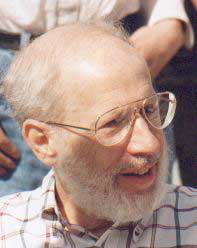
\includegraphics[width=1.5in]{Kruskal.png}
 \caption{ Joseph Kruskal} 
\end{figure}
} 

%
%
%
%\item 
%For graph $G$, we first construct its {\sc graphic matroid} $M_{G}=( S_G, {L} _G)$ as follows: 
%\begin{enumerate}
% \item {\sc Ground set: }  $S_G = E$, the set of edges; 
% \item {\sc Independent subsets:}  $A \in \mathcal{L}_G$ iff $A$ is acyclic. (Intuition: $A$ forms a forest, i.e.  a set of trees.)
% \item Weight: $w(e) = W_{max} - C(e)$, where $W_{max}$ is a large number to guarantee $w(e) > 0 $; 
%\end{enumerate}
%
%\item  
%Since $M_{G}$ is a matroid, the general {\sc Matroid\_Greedy} algorithm also applies: Kruskal's algorithm.
%\end{itemize}
%}

\frame{
\frametitle{ Kruskal's algorithm   [1956]}

{\sc MST-Kruskal}$( G, W )$
\begin{algorithmic}[1]
\STATE{ $F = \{ \}; $} 
\FORALL{ vertex $v \in V$ } 
\STATE{ {\sc MakeSet}$( v )$; }
\ENDFOR
\STATE\textcolor{red}{ sort the edges of $E$ into nondecreasing order by weight $W$; }
\FOR{ each edge $(u, v) \in E$ in the order } 
\IF { {\sc FindSet}$( u )$ $\neq$ {\sc FindSet}$( v )$ } 
\STATE $F = F \cup \{ ( u , v ) \};$ 
\STATE{{\sc Union} $( u, v )$; } 
\ENDIF
\ENDFOR
\end{algorithmic}

Here,  {\sc Union-Find} structure is used to detect whether a set of edges form a cycle. 

%(See extra slides for {\sc Union-Find} data structure, and a demo of Kruskal algorithm)
} 



\frame{
\frametitle{Kruskal's  MST algorithm: an example}

\begin{figure}

\begin{tikzpicture}[scale=0.9, auto,swap]

%problem 
     
    \foreach \pos/\name in {{(0,1)/s}, {(1.5,1)/a}, {(1.8, -0.8)/b}, {(0,-2.7)/c}, {(4.4 ,1)/d}, {(3.6,-2)/e}, {(5,-1.5)/f},{(6.5,-2.7)/t}}
        \node[middlevertex,fill=blue!20] (\name) at \pos {$\name$};
        
    \foreach \source/\dest/\weight in {s/a/9, s/b/14, s/c/15, a/d/24, b/d/18, b/e/30, c/e/20, d/e/2, e/f/11, e/t/16, f/t/6, d/t/19, c/t/44} 
                \draw[-, thick] (\source) -- node[above]{\small $\weight$} (\dest);
%initilization 
\pause
   \node[ultra thick, blue] at (3, 4) {Step 1}; 
  \node[ultra thick] at (3, 3) {Disjoint sets: $\{a\}, \{b\},\{c\},\{d\},\{e\},\{f\},\{s\},\{t\}$}; 
  \node[ultra thick] at (3, 3.5) {Edge weight: $\textcolor{green}{2}, 6, 9, 11, 14, 15, 16, 18, 19, 20, 24, 30, 44$}; 
%step 1
\pause
  \node[ ultra thick, green] at (8, 1) { {\sc Find}($d$) returns $\{d\}$}; 
  \node[ ultra thick, green] at (8, 0.5) { {\sc Find}($e$) returns $\{e\}$}; 
\pause
  \node[ ultra thick, green] at (8,  0.0) { {\sc Union}($d, e$)}; 
  
\pause  %clear and redraw
   \draw[fill=white,draw=white] (-2.7, 5) rectangle (10.5, -8); 
   \node[ultra thick, blue] at (3, 4) {Step 1}; 
  \node[ultra thick] at (3, 3) {Disjoint sets: $\{a\}, \{b\},\{c\},\{d, e\},\{f\},\{s\},\{t\}$}; 
  \node[ultra thick] at (3, 3.5) {Edge weight: $\textcolor{green}{2}, 6, 9, 11, 14, 15, 16, 18, 19, 20, 24, 30, 44$}; 
     
    \foreach \pos/\name in {{(0,1)/s}, {(1.5,1)/a}, {(1.8, -0.8)/b}, {(0,-2.7)/c}, {(4.4 ,1)/d}, {(3.6,-2)/e}, {(5,-1.5)/f},{(6.5,-2.7)/t}}
        \node[middlevertex,fill=blue!20] (\name) at \pos {$\name$};
        
    \foreach \source/\dest/\weight in {s/a/9, s/b/14, s/c/15, a/d/24, b/d/18, b/e/30, c/e/20, d/e/2, e/f/11, e/t/16, f/t/6, d/t/19, c/t/44} 
                \draw[-, thick] (\source) -- node[above]{\small $\weight$} (\dest);
    \foreach \source/\dest/\weight in { d/e/}   
  		\draw[-, ultra thick, red] (\source) -- node[above]{\small $\weight$} (\dest);

%step 2
\pause  %clear and redraw
   \draw[fill=white,draw=white] (-2.7, 5) rectangle (10.5, -8); 
   \node[ultra thick, blue] at (3, 4) {Step 2}; 
  \node[ultra thick] at (3, 3) {Disjoint sets: $\{a\}, \{b\},\{c\},\{d, e\},\{f\},  \{s\}, \{t\} $}; 
  \node[ultra thick] at (3, 3.5) {Edge weight: $2, \textcolor{green}{6}, 9, 11, 14, 15, 16, 18, 19, 20, 24, 30, 44$}; 
     
    \foreach \pos/\name in {{(0,1)/s}, {(1.5,1)/a}, {(1.8, -0.8)/b}, {(0,-2.7)/c}, {(4.4 ,1)/d}, {(3.6,-2)/e}, {(5,-1.5)/f},{(6.5,-2.7)/t}}
        \node[middlevertex,fill=blue!20] (\name) at \pos {$\name$};
        
    \foreach \source/\dest/\weight in {s/a/9, s/b/14, s/c/15, a/d/24, b/d/18, b/e/30, c/e/20, d/e/2, e/f/11, e/t/16, f/t/6, d/t/19, c/t/44} 
                \draw[-, thick] (\source) -- node[above]{\small $\weight$} (\dest);
    \foreach \source/\dest/\weight in { d/e/ }   
  		\draw[-, ultra thick, red] (\source) -- node[above]{\small $\weight$} (\dest);

\pause
  \node[ ultra thick, green] at (8, 1) { {\sc Find}($f$) returns $\{f\}$}; 
  \node[ ultra thick, green] at (8, 0.5) { {\sc Find}($t$) returns $\{t\}$}; 
\pause
  \node[ ultra thick, green] at (8,  0.0) { {\sc Union}($f, t$)}; 
  
\pause  %clear and redraw
   \draw[fill=white,draw=white] (-2.7, 5) rectangle (10.5, -8); 
   \node[ultra thick, blue] at (3, 4) {Step 2}; 
  \node[ultra thick] at (3, 3) {Disjoint sets: $\{a\}, \{b\},\{c\},\{d, e\},\{f, t\},\{s\} $}; 
  \node[ultra thick] at (3, 3.5) {Edge weight: $2, \textcolor{green}{6}, 9, 11, 14, 15, 16, 18, 19, 20, 24, 30, 44$}; 
     
    \foreach \pos/\name in {{(0,1)/s}, {(1.5,1)/a}, {(1.8, -0.8)/b}, {(0,-2.7)/c}, {(4.4 ,1)/d}, {(3.6,-2)/e}, {(5,-1.5)/f},{(6.5,-2.7)/t}}
        \node[middlevertex,fill=blue!20] (\name) at \pos {$\name$};
        
    \foreach \source/\dest/\weight in {s/a/9, s/b/14, s/c/15, a/d/24, b/d/18, b/e/30, c/e/20, d/e/2, e/f/11, e/t/16, f/t/6, d/t/19, c/t/44} 
                \draw[-, thick] (\source) -- node[above]{\small $\weight$} (\dest);
    \foreach \source/\dest/\weight in { d/e/, f/t/ }   
  		\draw[-, ultra thick, red] (\source) -- node[above]{\small $\weight$} (\dest);
  

%step 3
\pause  %clear and redraw
   \draw[fill=white,draw=white] (-2.7, 5) rectangle (10.5, -8); 
   \node[ultra thick, blue] at (3, 4) {Step 3}; 
  \node[ultra thick] at (3, 3) {Disjoint sets: $\{a\}, \{b\},\{c\},\{d, e\},\{f, t\},\{s\} $}; 
  \node[ultra thick] at (3, 3.5) {Edge weight: $2, 6, \textcolor{green}{9}, 11, 14, 15, 16, 18, 19, 20, 24, 30, 44$}; 
     
    \foreach \pos/\name in {{(0,1)/s}, {(1.5,1)/a}, {(1.8, -0.8)/b}, {(0,-2.7)/c}, {(4.4 ,1)/d}, {(3.6,-2)/e}, {(5,-1.5)/f},{(6.5,-2.7)/t}}
        \node[middlevertex,fill=blue!20] (\name) at \pos {$\name$};
        
    \foreach \source/\dest/\weight in {s/a/9, s/b/14, s/c/15, a/d/24, b/d/18, b/e/30, c/e/20, d/e/2, e/f/11, e/t/16, f/t/6, d/t/19, c/t/44} 
                \draw[-, thick] (\source) -- node[above]{\small $\weight$} (\dest);
    \foreach \source/\dest/\weight in { d/e/, f/t/ }   
  		\draw[-, ultra thick, red] (\source) -- node[above]{\small $\weight$} (\dest);

\pause
  \node[ ultra thick, green] at (8, 1) { {\sc Find}($s$) returns $\{s\}$}; 
  \node[ ultra thick, green] at (8, 0.5) { {\sc Find}($a$) returns $\{a\}$}; 
\pause
  \node[ ultra thick, green] at (8,  0.0) { {\sc Union}($s, a$)}; 
  
\pause  %clear and redraw
   \draw[fill=white,draw=white] (-2.7, 5) rectangle (10.5, -8); 
   \node[ultra thick, blue] at (3, 4) {Step 3}; 
  \node[ultra thick] at (3, 3) {Disjoint sets: $\{a, s\}, \{b\},\{c\},\{d, e\},\{f, t\}$}; 
  \node[ultra thick] at (3, 3.5) {Edge weight: $2, 6, \textcolor{green}{9}, 11, 14, 15, 16, 18, 19, 20, 24, 30, 44$}; 
     
    \foreach \pos/\name in {{(0,1)/s}, {(1.5,1)/a}, {(1.8, -0.8)/b}, {(0,-2.7)/c}, {(4.4 ,1)/d}, {(3.6,-2)/e}, {(5,-1.5)/f},{(6.5,-2.7)/t}}
        \node[middlevertex,fill=blue!20] (\name) at \pos {$\name$};
        
    \foreach \source/\dest/\weight in {s/a/9, s/b/14, s/c/15, a/d/24, b/d/18, b/e/30, c/e/20, d/e/2, e/f/11, e/t/16, f/t/6, d/t/19, c/t/44} 
                \draw[-, thick] (\source) -- node[above]{\small $\weight$} (\dest);
    \foreach \source/\dest/\weight in { d/e/, f/t/, a/s/}   
  		\draw[-, ultra thick, red] (\source) -- node[above]{\small $\weight$} (\dest);


%step 4
\pause  %clear and redraw
   \draw[fill=white,draw=white] (-2.7, 5) rectangle (10.5, -8); 
   \node[ultra thick, blue] at (3, 4) {Step 4}; 
  \node[ultra thick] at (3, 3) {Disjoint sets: $\{a, s\}, \{b\},\{c\},\{d, e\},\{f, t\}$}; 
  \node[ultra thick] at (3, 3.5) {Edge weight: $2, 6, 9, \textcolor{green}{11}, 14, 15, 16, 18, 19, 20, 24, 30, 44$}; 
     
    \foreach \pos/\name in {{(0,1)/s}, {(1.5,1)/a}, {(1.8, -0.8)/b}, {(0,-2.7)/c}, {(4.4 ,1)/d}, {(3.6,-2)/e}, {(5,-1.5)/f},{(6.5,-2.7)/t}}
        \node[middlevertex,fill=blue!20] (\name) at \pos {$\name$};
        
    \foreach \source/\dest/\weight in {s/a/9, s/b/14, s/c/15, a/d/24, b/d/18, b/e/30, c/e/20, d/e/2, e/f/11, e/t/16, f/t/6, d/t/19, c/t/44} 
                \draw[-, thick] (\source) -- node[above]{\small $\weight$} (\dest);
    \foreach \source/\dest/\weight in { d/e/, f/t/, a/s/}   
  		\draw[-, ultra thick, red] (\source) -- node[above]{\small $\weight$} (\dest);

\pause
  \node[ ultra thick, green] at (7, 1) { {\sc Find}($e$) returns $\{d, e\}$}; 
  \node[ ultra thick, green] at (7, 0.5) { {\sc Find}($f$) returns $\{f, t\}$}; 
\pause
  \node[ ultra thick, green] at (7,  0.0) { {\sc Union}($e, f$)}; 
  
\pause  %clear and redraw
   \draw[fill=white,draw=white] (-2.7, 5) rectangle (10.5, -8); 
   \node[ultra thick, blue] at (3, 4) {Step 4}; 
  \node[ultra thick] at (3, 3) {Disjoint sets: $\{a, s\}, \{b\},\{c\},\{d, e, f, t\}$}; 
  \node[ultra thick] at (3, 3.5) {Edge weight: $2, 6, 9, \textcolor{green}{11}, 14, 15, 16, 18, 19, 20, 24, 30, 44$}; 
     
    \foreach \pos/\name in {{(0,1)/s}, {(1.5,1)/a}, {(1.8, -0.8)/b}, {(0,-2.7)/c}, {(4.4 ,1)/d}, {(3.6,-2)/e}, {(5,-1.5)/f},{(6.5,-2.7)/t}}
        \node[middlevertex,fill=blue!20] (\name) at \pos {$\name$};
        
    \foreach \source/\dest/\weight in {s/a/9, s/b/14, s/c/15, a/d/24, b/d/18, b/e/30, c/e/20, d/e/2, e/f/11, e/t/16, f/t/6, d/t/19, c/t/44} 
                \draw[-, thick] (\source) -- node[above]{\small $\weight$} (\dest);
    \foreach \source/\dest/\weight in { d/e/, f/t/, a/s/, e/f/}   
  		\draw[-, ultra thick, red] (\source) -- node[above]{\small $\weight$} (\dest);
                  
 
 
%step 5
\pause  %clear and redraw
   \draw[fill=white,draw=white] (-2.7, 5) rectangle (10.5, -8); 
   \node[ultra thick, blue] at (3, 4) {Step 5}; 
  \node[ultra thick] at (3, 3) {Disjoint sets: $\{a, s\}, \{b\},\{c\},\{d, e, f, t\}$}; 
  \node[ultra thick] at (3, 3.5) {Edge weight: $2, 6, 9, 11, \textcolor{green}{14}, 15, 16, 18, 19, 20, 24, 30, 44$}; 
     
    \foreach \pos/\name in {{(0,1)/s}, {(1.5,1)/a}, {(1.8, -0.8)/b}, {(0,-2.7)/c}, {(4.4 ,1)/d}, {(3.6,-2)/e}, {(5,-1.5)/f},{(6.5,-2.7)/t}}
        \node[middlevertex,fill=blue!20] (\name) at \pos {$\name$};
        
    \foreach \source/\dest/\weight in {s/a/9, s/b/14, s/c/15, a/d/24, b/d/18, b/e/30, c/e/20, d/e/2, e/f/11, e/t/16, f/t/6, d/t/19, c/t/44} 
                \draw[-, thick] (\source) -- node[above]{\small $\weight$} (\dest);
    \foreach \source/\dest/\weight in { d/e/, f/t/, a/s/, e/f/}   
  		\draw[-, ultra thick, red] (\source) -- node[above]{\small $\weight$} (\dest);

\pause
  \node[ ultra thick, green] at (7, 1) { {\sc Find}($s$) returns $\{s, a\}$}; 
  \node[ ultra thick, green] at (7, 0.5) { {\sc Find}($b$) returns $\{b\}$}; 
\pause
  \node[ ultra thick, green] at (7,  0.0) { {\sc Union}($s, b$)}; 
  
\pause  %clear and redraw
   \draw[fill=white,draw=white] (-2.7, 5) rectangle (10.5, -8); 
   \node[ultra thick, blue] at (3, 4) {Step 5}; 
  \node[ultra thick] at (3, 3) {Disjoint sets: $\{a, s, b\},\{c\},\{d, e, f, t\}$}; 
  \node[ultra thick] at (3, 3.5) {Edge weight: $2, 6, 9, 11, \textcolor{green}{14}, 15, 16, 18, 19, 20, 24, 30, 44$}; 
     
    \foreach \pos/\name in {{(0,1)/s}, {(1.5,1)/a}, {(1.8, -0.8)/b}, {(0,-2.7)/c}, {(4.4 ,1)/d}, {(3.6,-2)/e}, {(5,-1.5)/f},{(6.5,-2.7)/t}}
        \node[middlevertex,fill=blue!20] (\name) at \pos {$\name$};
        
    \foreach \source/\dest/\weight in {s/a/9, s/b/14, s/c/15, a/d/24, b/d/18, b/e/30, c/e/20, d/e/2, e/f/11, e/t/16, f/t/6, d/t/19, c/t/44} 
                \draw[-, thick] (\source) -- node[above]{\small $\weight$} (\dest);
    \foreach \source/\dest/\weight in { d/e/, f/t/, a/s/, e/f/, s/b/}   
  		\draw[-, ultra thick, red] (\source) -- node[above]{\small $\weight$} (\dest);
            
  
  
%step 6
\pause  %clear and redraw
   \draw[fill=white,draw=white] (-2.7, 5) rectangle (10.5, -8); 
   \node[ultra thick, blue] at (3, 4) {Step 6}; 
  \node[ultra thick] at (3, 3) {Disjoint sets: $\{a, s, b\},\{c\},\{d, e, f, t\}$}; 
  \node[ultra thick] at (3, 3.5) {Edge weight: $2, 6, 9, 11, 14, \textcolor{green}{15}, 16, 18, 19, 20, 24, 30, 44$}; 
     
    \foreach \pos/\name in {{(0,1)/s}, {(1.5,1)/a}, {(1.8, -0.8)/b}, {(0,-2.7)/c}, {(4.4 ,1)/d}, {(3.6,-2)/e}, {(5,-1.5)/f},{(6.5,-2.7)/t}}
        \node[middlevertex,fill=blue!20] (\name) at \pos {$\name$};
        
    \foreach \source/\dest/\weight in {s/a/9, s/b/14, s/c/15, a/d/24, b/d/18, b/e/30, c/e/20, d/e/2, e/f/11, e/t/16, f/t/6, d/t/19, c/t/44} 
                \draw[-, thick] (\source) -- node[above]{\small $\weight$} (\dest);
    \foreach \source/\dest/\weight in { d/e/, f/t/, a/s/, e/f/, s/b/}   
  		\draw[-, ultra thick, red] (\source) -- node[above]{\small $\weight$} (\dest);
            

\pause
  \node[ ultra thick, green] at (7, 1) { {\sc Find}($s$) returns $\{s, a, b\}$}; 
  \node[ ultra thick, green] at (7, 0.5) { {\sc Find}($c$) returns $\{c\}$}; 
\pause
  \node[ ultra thick, green] at (7,  0.0) { {\sc Union}($s, c$)}; 
  
\pause  %clear and redraw
   \draw[fill=white,draw=white] (-2.7, 5) rectangle (10.5, -8); 
   \node[ultra thick, blue] at (3, 4) {Step 6}; 
  \node[ultra thick] at (3, 3) {Disjoint sets: $\{a, s, b, c\},\{d, e, f, t\}$}; 
  \node[ultra thick] at (3, 3.5) {Edge weight: $2, 6, 9, 11, 14, \textcolor{green}{15}, 16, 18, 19, 20, 24, 30, 44$}; 
     
    \foreach \pos/\name in {{(0,1)/s}, {(1.5,1)/a}, {(1.8, -0.8)/b}, {(0,-2.7)/c}, {(4.4 ,1)/d}, {(3.6,-2)/e}, {(5,-1.5)/f},{(6.5,-2.7)/t}}
        \node[middlevertex,fill=blue!20] (\name) at \pos {$\name$};
        
    \foreach \source/\dest/\weight in {s/a/9, s/b/14, s/c/15, a/d/24, b/d/18, b/e/30, c/e/20, d/e/2, e/f/11, e/t/16, f/t/6, d/t/19, c/t/44} 
                \draw[-, thick] (\source) -- node[above]{\small $\weight$} (\dest);
    \foreach \source/\dest/\weight in { d/e/, f/t/, a/s/, e/f/, s/b/, s/c/}   
  		\draw[-, ultra thick, red] (\source) -- node[above]{\small $\weight$} (\dest);
  
  
%step 7
\pause  %clear and redraw
   \draw[fill=white,draw=white] (-2.7, 5) rectangle (10.5, -8); 
   \node[ultra thick, blue] at (3, 4) {Step 7}; 
  \node[ultra thick] at (3, 3) {Disjoint sets: $\{a, s, b, c\},\{d, e, f, t\}$}; 
  \node[ultra thick] at (3, 3.5) {Edge weight: $2, 6, 9, 11, 14, 15, \textcolor{green}{16}, 18, 19, 20, 24, 30, 44$}; 
     
    \foreach \pos/\name in {{(0,1)/s}, {(1.5,1)/a}, {(1.8, -0.8)/b}, {(0,-2.7)/c}, {(4.4 ,1)/d}, {(3.6,-2)/e}, {(5,-1.5)/f},{(6.5,-2.7)/t}}
        \node[middlevertex,fill=blue!20] (\name) at \pos {$\name$};
        
    \foreach \source/\dest/\weight in {s/a/9, s/b/14, s/c/15, a/d/24, b/d/18, b/e/30, c/e/20, d/e/2, e/f/11, e/t/16, f/t/6, d/t/19, c/t/44} 
                \draw[-, thick] (\source) -- node[above]{\small $\weight$} (\dest);
    \foreach \source/\dest/\weight in { d/e/, f/t/, a/s/, e/f/, s/b/, s/c/}   
  		\draw[-, ultra thick, red] (\source) -- node[above]{\small $\weight$} (\dest);
		
\pause
  \node[ ultra thick, green] at (7, 1) { {\sc Find}($e$) returns $\{d, e, f, t\}$}; 
  \node[ ultra thick, green] at (7, 0.5) { {\sc Find}($t$) returns $\{d, e, f, t\}$}; 
  \node[ ultra thick, red] at (7,  0.0) { Same set!}; 
 
 \pause 
%redraw  
   \draw[fill=white,draw=white] (-2.7, 5) rectangle (10.5, -8); 
   \node[ultra thick, blue] at (3, 4) {Step 8}; 
  \node[ultra thick] at (3, 3) {Disjoint sets: $\{a, s, b, c\},\{d, e, f, t\}$}; 
  \node[ultra thick] at (3, 3.5) {Edge weight: $2, 6, 9, 11, 14, 15, 16, \textcolor{green}{18}, 19, 20, 24, 30, 44$}; 
     
    \foreach \pos/\name in {{(0,1)/s}, {(1.5,1)/a}, {(1.8, -0.8)/b}, {(0,-2.7)/c}, {(4.4 ,1)/d}, {(3.6,-2)/e}, {(5,-1.5)/f},{(6.5,-2.7)/t}}
        \node[middlevertex,fill=blue!20] (\name) at \pos {$\name$};
        
    \foreach \source/\dest/\weight in {s/a/9, s/b/14, s/c/15, a/d/24, b/d/18, b/e/30, c/e/20, d/e/2, e/f/11, e/t/16, f/t/6, d/t/19, c/t/44} 
                \draw[-, thick] (\source) -- node[above]{\small $\weight$} (\dest);
    \foreach \source/\dest/\weight in { d/e/, f/t/, a/s/, e/f/, s/b/, s/c/}   
  		\draw[-, ultra thick, red] (\source) -- node[above]{\small $\weight$} (\dest);

\pause
  \node[ ultra thick, green] at (7, 1) { {\sc Find}($b$) returns $\{a, s, b, c\}$}; 
  \node[ ultra thick, green] at (7, 0.5) { {\sc Find}($d$) returns $\{d, e, f, t\}$}; 
\pause
  \node[ ultra thick, green] at (7,  0.0) {  {\sc Union}($b, d$) };     
  
\pause  %clear and redraw
   \draw[fill=white,draw=white] (-2.7, 5) rectangle (10.5, -8); 
   \node[ultra thick, blue] at (3, 4) {Step 8}; 
  \node[ultra thick] at (3, 3) {Disjoint sets: $\{a, s, b, c, d, e, f, t\}$}; 
  \node[ultra thick] at (3, 3.5) {Edge weight: $2, 6, 9, 11, 14, 15, 16, \textcolor{green}{18}, 19, 20, 24, 30, 44$}; 
     
    \foreach \pos/\name in {{(0,1)/s}, {(1.5,1)/a}, {(1.8, -0.8)/b}, {(0,-2.7)/c}, {(4.4 ,1)/d}, {(3.6,-2)/e}, {(5,-1.5)/f},{(6.5,-2.7)/t}}
        \node[middlevertex,fill=blue!20] (\name) at \pos {$\name$};
        
    \foreach \source/\dest/\weight in {s/a/9, s/b/14, s/c/15, a/d/24, b/d/18, b/e/30, c/e/20, d/e/2, e/f/11, e/t/16, f/t/6, d/t/19, c/t/44} 
                \draw[-, thick] (\source) -- node[above]{\small $\weight$} (\dest);
    \foreach \source/\dest/\weight in { d/e/, f/t/, a/s/, e/f/, s/b/, s/c/, b/d/}   
  		\draw[-, ultra thick, red] (\source) -- node[above]{\small $\weight$} (\dest);
    \node[ ultra thick, red] at (7,  0.0) {  Done! };     
               
  
   
\end{tikzpicture} 
\end{figure}    

}


\frame{
	\frametitle{ Time complexity of {\sc Kruskal's MST} algorithm} 

  \begin{table}
  \begin{tabular}{crrrr}
  \hline  \hline
  Operation & Array  & Tree  & Link-by-size  & Link-by-size +  \\
            &    &    &   & path compression \\
  \hline
   {\sc MakeSet} & $ 1 $ &  $1$  & $ 1 $ & $1$  \\ 
  {\sc Find} & $ 1 $ &  $n$  & $ \log n $ & $lg^* n$  \\ 
  {\sc Union} & $ n $ &  $1$  & $ \log n $ & $lg^* n$  \\ 
  \hline 
  {\sc Kruskal's MST} & $ O(n^2) $ &  $ O(mn) $  & $ O( m \log n ) $ & $ O( m  lg^* n) $  \\ 
  \hline \hline 
  \end{tabular} 
  \end{table}
{\sc Kruskal's MST} algorithm: $n$ {\sc MakeSet}, $n-1$ {\sc Union}, and $m$ {\sc Find}. 
}

\end{document}
